\documentclass[11pt,a4paper,oneside]{report}
\usepackage{amsmath,amssymb,calc,ifthen}
\usepackage{float}
%\usepackage{cancel}
\usepackage[table,usenames,dvipsnames]{xcolor} % for coloured cells in tables
\usepackage{tikz}
% Allows us to click on links and references!
\usepackage{hyperref}
\usepackage{url}
\hypersetup{
colorlinks,
citecolor=black,
filecolor=black,
linkcolor=black,
urlcolor=black
}
% Nice package for plotting graphs
% See excellent guide:
% http://www.tug.org/TUGboat/tb31-1/tb97wright-pgfplots.pdf
\usetikzlibrary{plotmarks,shapes}
\usepackage{amsmath,graphicx}
\usepackage{epstopdf}
\usepackage{caption}
\usepackage{subcaption}
% highlight - useful for TODOs and similar
\usepackage{color}
\newcommand{\hilight}[1]{\colorbox{yellow}{#1}}
\newcommand\ci{\perp\!\!\!\perp} % perpendicular sign
\newcommand*\rfrac[2]{{}^{#1}\!/_{#2}} % diagonal fraction
\newcommand\SLASH{\char`\\}
\usepackage{listings}
% margin size
\usepackage[margin=1in]{geometry}
\tikzstyle{state}=[circle,thick,draw=black, align=center, minimum size=2.1cm,
inner sep=0]
\tikzstyle{vertex}=[circle,thick,draw=black]
\tikzstyle{terminal}=[rectangle,thick,draw=black]
\tikzstyle{edge} = [draw,thick]
\tikzstyle{lo} = [edge,dotted]
\tikzstyle{hi} = [edge]
\tikzstyle{trans} = [edge,->]
\definecolor{mygreen}{rgb}{0,0.6,0}
\definecolor{mygray}{rgb}{0.5,0.5,0.5}
\definecolor{mymauve}{rgb}{0.58,0,0.82}
\DeclareMathOperator*{\argmin}{arg\,min}
\DeclareMathOperator*{\argmax}{arg\,max}
\lstset{ %
backgroundcolor=\color{white}, % choose the background color; you must add
%\usepackage{color} or \usepackage{xcolor}
basicstyle=\footnotesize, % the size of the fonts that are used for the
%code
breakatwhitespace=false, % sets if automatic breaks should only happen
%at whitespace
breaklines=true, % sets automatic line breaking
captionpos=b, % sets the caption-position to bottom
commentstyle=\color{mygreen}, % comment style
deletekeywords={...}, % if you want to delete keywords from the
%given language
escapeinside={\%*}{*)}, % if you want to add LaTeX within your code
extendedchars=true, % lets you use non-ASCII characters; for
%8-bits encodings only, does not work with UTF-8
frame=single, % adds a frame around the code
keepspaces=true, % keeps spaces in text, useful for keeping
%indentation of code (possibly needs columns=flexible)
keywordstyle=\color{blue}, % keyword style
language=Octave, % the language of the code
morekeywords={*,...}, % if you want to add more keywords to the set
numbers=left, % where to put the line-numbers; possible
%values are (none, left, right)
numbersep=5pt, % how far the line-numbers are from the code
numberstyle=\tiny\color{mygray}, % the style that is used for the line-numbers
rulecolor=\color{black}, % if not set, the frame-color may be changed
%on line-breaks within not-black text (e.g. comments (green here))
showspaces=false, % show spaces everywhere adding particular
%underscores; it overrides 'showstringspaces'
showstringspaces=false, % underline spaces within strings only
showtabs=false, % show tabs within strings adding particular
%underscores
stepnumber=2, % the step between two line-numbers. If it's
%1, each line will be numbered
stringstyle=\color{mymauve}, % string literal style
tabsize=2, % sets default tabsize to 2 spaces
title=\lstname % show the filename of files included with
%\lstinputlisting; also try caption instead of title
}
\title{Computational Modelling for Biomedical Imaging - Coursework 1}
\author{
Razvan Valentin Marinescu\\
Student Number: 14060166\\
\texttt{razvan.marinescu.14@ucl.ac.uk}
}
\begin{document}
\belowdisplayskip=12pt plus 3pt minus 9pt
\belowdisplayshortskip=7pt plus 3pt minus 4pt
\maketitle{}

\section*{Q1.1.1}
\begin{figure}[H]
\centering
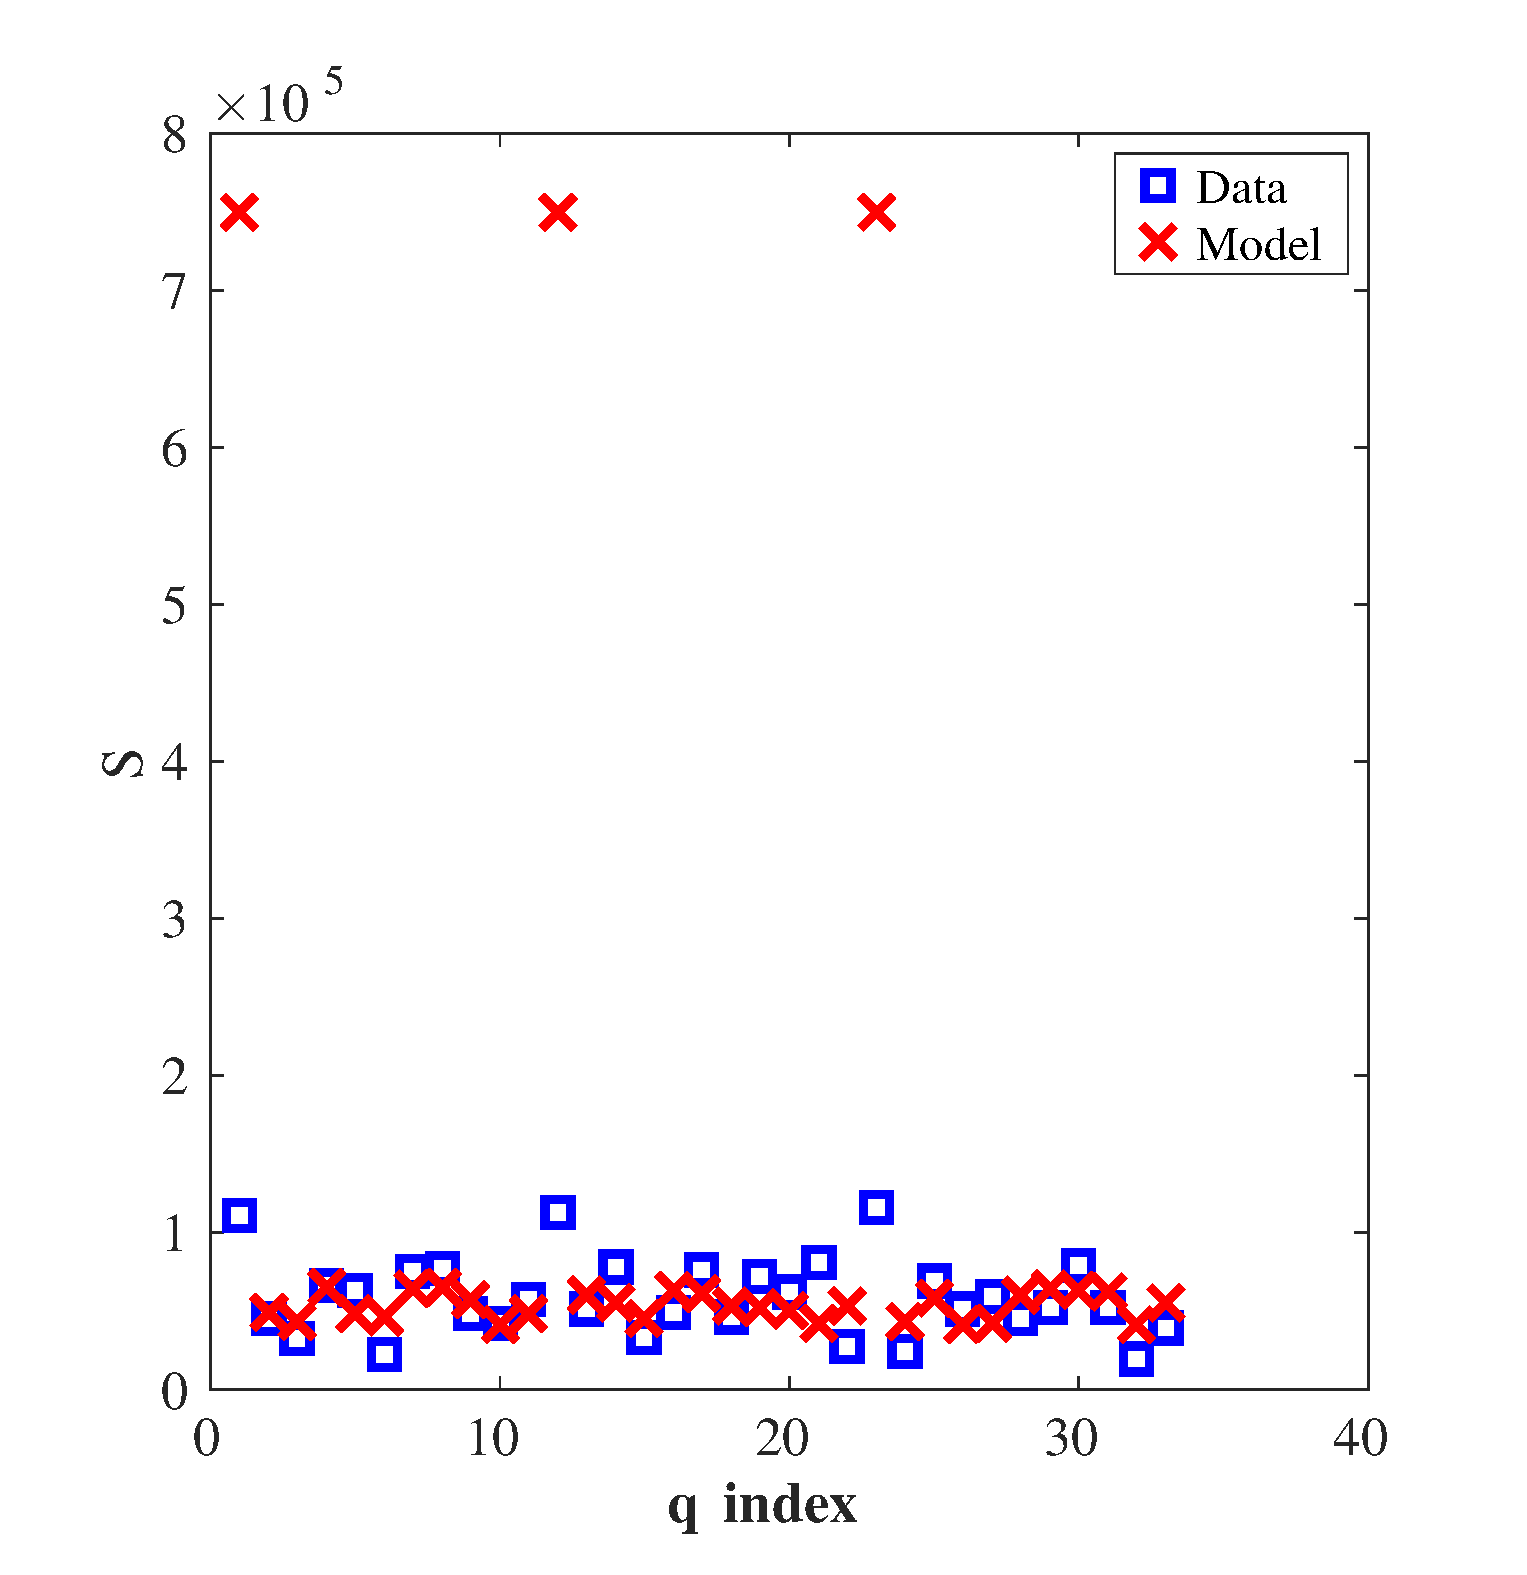
\includegraphics[scale=0.5]{figures/q111.eps}
\caption{Data points for the voxel at position $(52,62,25)$}
\end{figure}


%Think about the quality of the fit you obtain above.  First, eyeball the fit 
%to the data by comparing the predictions from the model with your fitted 
%parameters to the actual measurements, as in the lectures. 

From eyeballing the data we notice that the fit is very poor, especially for the 3 entries where the b-value is 0, having a $\Delta S > 7 * 10^5$. The other entries don't fit the data well either.

%Then, is the final 
%value of RESNORM above the kind of value for the sum of square differences we 
%expect?  

The final value of RESNORM (1.2242e+12) is clearly above the kind of value we would normally expect. The fit is poor probably because the search strategy got stuck in a local minima.

%The standard deviation of the noise on each measurement of this data 
%set is somewhere in the range 5000-­‐6000.  Given that, what would you expect a 
%typical value of RESNORM to be? 
 

The expected value of RESNORM would be given by the formula:
$$E\left[\sum_{i=1}^{33} (X_i - \bar{X}_i)^2\right] = E\left[\sum_{i=1}^{33} \sigma_i^2\right] = 33 * \sigma^2 $$
Since sigma is between 5000-6000 this means that $ 8.25*10^8 < RESNORM < 1.188 * 10^9$.

%Are the parameter values sensible given the 
%quantities they represent?	

Some of the parameter values we obtain are not sensible. For example, the value of $f$ is negative, meaning that we give too much weight to the $S_E$ component of the model, extrapolating outside the intended $(0,1)$ range. The value of S0 is also really high, when in fact it should be around $1.1 * 10^5$. 


\section*{Q1.1.2}
%% TODO: insert picture (maybe)

We did the following transformations to ensure the parameters stayed within the required bounds:
\begin{itemize}
 \item $S0 \to S0^2$
 \item $d \to d^2$
 \item $f \to atan(f)$
\end{itemize}

We apply the inverse transformation at the beginning in order to maintain the starting point. This time the algorithm converges to the following parameters: $S0 = 113204, d=21521 f=-1.51, \theta=-12.89,  \phi=-47.31$ with a RESNORM of 9.48e+10. There is an 11-fold improvement from the unconstrained version and by eyeballing the data we find that the value for $S0$ is what we expected. However, the $d$ parameter is too large while $f$ is really close to zero, suggesting that the whole brain is mostly made of balls, with almost no sticks. The improvement in the SSD value is because of the fact that parameters were constrained to physically realistic bounds. However, the expected RESNORM (around $10^9$) is still much lower that out current value, suggesting that the algorithm again got stuck in a local minima.

\section*{Q1.1.3}

\end{document}





















